% !TEX root       = ./type_name.tex
% !TEX program    = pdflatex
% !TEX encoding   = utf-8
% !TEX spellcheck = de_DE_frami
%=======================================================================

%\chapter{Introduction}\label{ch:einleitung}
\chapter{Background}\label{ch:Background}
\sffamily{}

This chapter discusses about the background to understand this thesis, it includes an introduction to software defined networking, explains 802.11 protocol, and a brief introduction on Hotspot 2.0 and BIC-IRAP project.

\section{Software Defined Networking \cite{SDN}}\label{sec:SDN}

SDN is nothing but the physical separation of the network control plane from the forwarding plane. The control plane consists of all the logic (or instructions) that the switch requires for correctly setting up a forwarding plane.

Traditionally, the vendor has the control over the instructions necessary for signaling since the devices run a proprietary firmware within the switch. This makes the devices non-interoperable with other vendors, thus hampering flexibility. Though most of these switches provide SNMP based management solution via Command Line Interface (CLI), they still do not allow the introduction of custom control plane function or protocol into the switch. This makes experimenting with new protocols cumbersome. Software Defined Networking aims to alleviate these problems by making the switched forwarding plane to be easily accessible remotely and modifiable using the OpenFlow protocol. Any third-party software can take advantage of this open protocol to manage and orchestrate an entire network.

SDN architecture generally has three components or groups of functionality as shown in the figure \ref{fig:sdn-architecture}.

\begin{itemize}
	\item \textbf{Application Layer:}  Consists of programs that communicate the behaviors and needed resources with the SDN controller via the application protocol interfaces (API’s). It can also build an abstracted view of the network by collecting information from the controller.
	\item \textbf{Control Layer:} This logical layer functions as a relay that sends the instructions or resources sent by the application layer to the networking components.
	\item \textbf{Infrastructure Layer:} This holds the SDN networking devices that control the forwarding and data processing capabilities of the network including the function to forward and process the data paths.
\end{itemize}

\begin{figure}
  \centering
  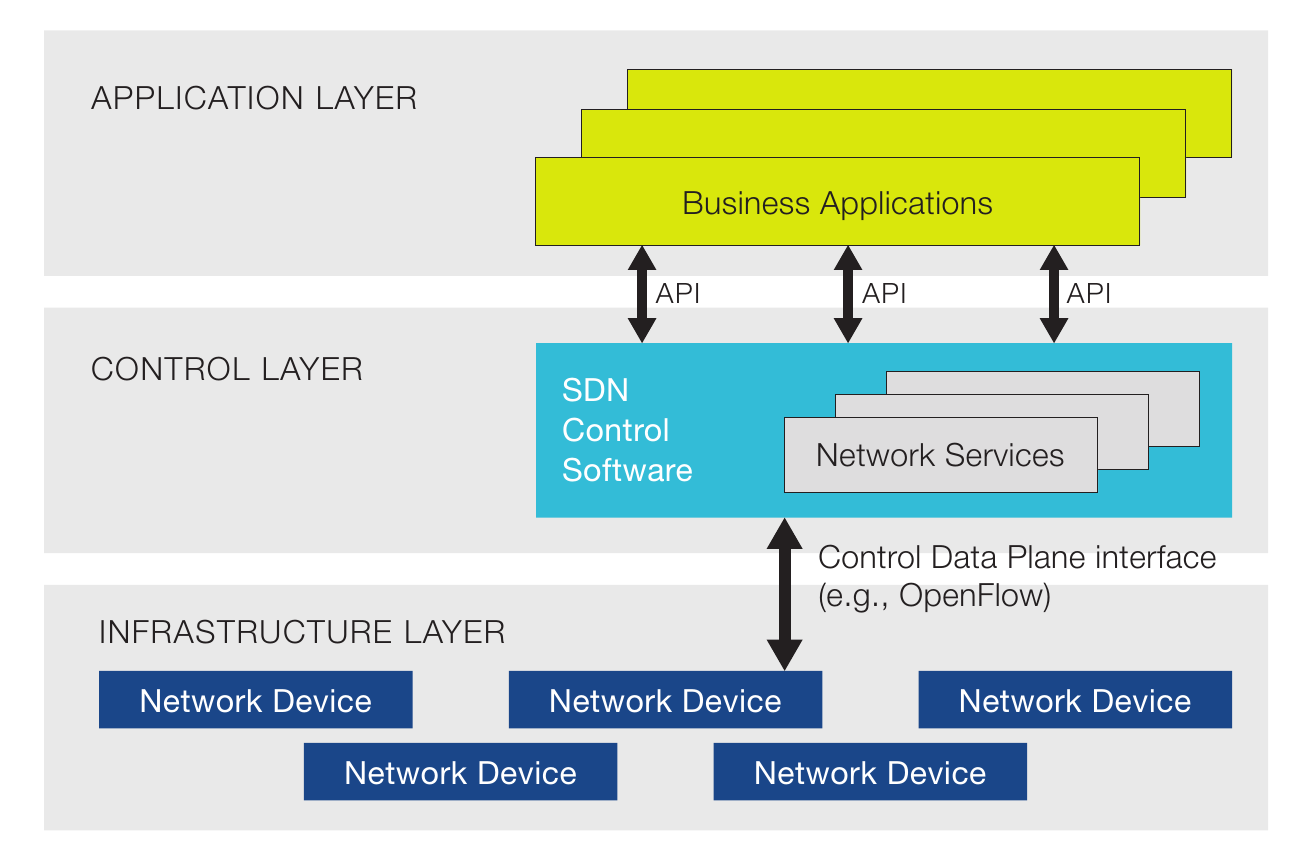
\includegraphics[width=1.0\linewidth]{sdn-architecture}
  \caption{SDN architecture diagram\cite{SDN:architecture}}
  \label{fig:sdn-architecture}
\end{figure}

\section{IEEE 802.11 MAC \cite{ieee2012802}}\label{sec:IEEE802.11}

The IEEE 802.11 Media Access Control Layer (MAC) \cite{ieee2012802} defines the protocol for stations to establish connections with each other and transmit data frames.
Medium access in 802.11 is performed by a distributed coordination function (DCF), which uses carrier sense multiple access with collision avoidance (CSMA/CA) to enable random medium access among all contending stations (STAs). Hence, it reduces the amount of collisions. Logically, the MAC is divided into two parts, an upper MAC, and a lower MAC. The upper MAC handles management frames, which include probe, authentication, association requests and their corresponding responses. The lower MAC handles control frames, which includes acknowledgement (ACK) frames, along with request-to-send (RTS) and clear-to-send (CTS) frames. The frames handled by the lower MAC have real-time constraints. For instance, ACK frame timeouts are within the order of micro-seconds. For this reason, control frames are handled and generated within hardware. Management frames, however, have softer time constraints, and can be handled in software locally (as is the case in Linux systems that use hostapd \cite{hostapd}), or remotely (as is the case when using a centralized WLAN controller \cite{RFC5412L97} ).

An 802.11 based wireless interface can operate under the following operating modes: STA (client), access point (AP), mesh, ad-hoc and item Monitor mode. The most common mode of operation is the infrastructure mode (which includes enterprise WLAN environments). In this mode of operation, clients connect to the AP using a series of message exchanges in a process called “association”. The decision on which AP to associate with is left entirely to the client. Clients learn about APs either passively through beacon frames that are periodically broadcasted by the access points, or actively by performing a probe scan. 

In a probe scan, clients first send out probe request frames over all channels. APs that receive these frames and are willing to accept a connection from a client respond with a probe response frame. All APs from which the client receives probe responses are candidates for the client to associate with. Next, the client sends an authentication frame, and waits for an authentication response from the AP. This is followed by the client sending an association request, and receiving an association response from the AP. If the network is operating in open authentication mode, the client is considered to be
associated at this point, and can now transmit data frames to be forwarded by the AP. If the AP is configured to use WPA, WPA2, or WPA2 Enterprise, the corresponding 802.1X \cite{hostapd} handshake is performed after the association phase before clients can forward data frames through the AP.


\section{Hotspot 2.0 \cite{Hotspot_2.0_Definition}} \label{Hotspot2.0}

It is a new wireless network standard that is designed to make connections to public Wi-Fi hotspots more easy and secure. They are already supported on many mobile devices running some of the popular operating systems such as Windows 10, Mac OS 10.9 or newer, Android 6.0 or newer, and iOS 7 or newer.

The main purpose of Hotspot 2.0 is to provide seamless mobility like cellular style “roaming” for Wi-Fi networks. The device will automatically connect to the available networks based on the networks partners on the home networks while roaming globally. This is made possible using the latest 802.11u \cite{IEEE802.11u} protocol designed for the same purpose. The organization WIFI Alliance also call this as Passpoint \cite{Passpoint}.